
%------------------------------------------------------------------------
%
%    Copyright (C) 1985-2020  Georg Umgiesser
%
%    This file is part of SHYFEM.
%
%    SHYFEM is free software: you can redistribute it and/or modify
%    it under the terms of the GNU General Public License as published by
%    the Free Software Foundation, either version 3 of the License, or
%    (at your option) any later version.
%
%    SHYFEM is distributed in the hope that it will be useful,
%    but WITHOUT ANY WARRANTY; without even the implied warranty of
%    MERCHANTABILITY or FITNESS FOR A PARTICULAR PURPOSE. See the
%    GNU General Public License for more details.
%
%    You should have received a copy of the GNU General Public License
%    along with SHYFEM. Please see the file COPYING in the main directory.
%    If not, see <http://www.gnu.org/licenses/>.
%
%    Contributions to this file can be found below in the revision log.
%
%------------------------------------------------------------------------
\newcommand{\Ttwoa}{\ref{FuncDesc}}
\subsection{AQUABC}
The model is focused on cyanobacteria and nitrogen fixation. It incorporates five groups of phytoplankton represented by six state variables: diatoms, non-nitrogen fixing cyanobacteria, nitrogen fixing cyanobacteria, nostacales, akinetes (representing a second group of nitrogen fixing cyanobacteria) and other planktonic algae. However it is a full ecological model containing one group of zooplankton, inorganic nutrients (C, N, P, Si), dissolved organic matter (DOC, DON, DOP), detrital particulate organic matter (POC, PON, POP) and other support variables (Alkalinity, Dissolved Oxygen and Biogenic Silicon in particulate form) as well. The list of the state variables are given in \ref{tab:table_aquabc}

\begin{table}[ht]
\caption{The list of state variables of pelagic model.}
\begin{tabular}{lcl} \hline
State Variable&	Unit \\
Total ammonia nitrogen &	gN·m-3 \\
Nitrate nitrogen	&gN·m-3\\
Orthophosphate phosphorus&	gP·m-3\\
Dissolved silicon&	gSi·m-3\\
Dissolved oxygen&	gO2·m-3\\
Diatoms carbon&	gC·m-3\\
Non-fixing cyanobacteria carbon&	gC·m-3\\
Fixing cyanobacteria carbon&	gC·m-3\\
Nostocates (vegetative-heterocyst cells) carbon	&gC·m-3\\
Nostocates (akinetes) carbon&	gC·m-3\\
Other planktonic algae carbon&	gC·m-3\\
Zooplankton carbon&	gC·m-3\\
Zooplankton nitrogen&	gN·m-3\\
Zooplankton phosphorus&	gP·m-3\\
Detrital particulate organic carbon&	gC·m-3\\
Detrital particulate organic nitrogen&	gN·m-3\\
Detrital particulate organic phosphorus	gP·m-3\\
Particulate silica&	gSi·m-3\\
Dissolved organic carbon&	gC·m-3\\
Dissolved organic nitrogen	&gN·m-3\\
Dissolved organic phosphorus&	gP·m-3\\
Dissolved inorganic carbon&	gC·m-3\\
Alkalinity	&moles/L \\
\hline
\end{tabular}
\label{tab:table_aquabc}
\end{table}

The phytoplankton groups interact with all of the state variables through several processes. The model assumes fixed stoichiometry for phytoplankton and variable stoichiometry for zooplankton. All phytoplankton undergo the same five main processes; where growth results in uptake of the relevant nutrients and incorporate them into phytoplankton biomass where
\begin{itemize}
\item Primary production incorporates free nutrients into phytoplankton biomass
\item Death converts the phytoplankton biomass to detrital particulate organic matter 
\item Excretion converts the phytoplankton biomass to dissolved organic matter
\item Respiration converts the phytoplankton biomass to inorganic nutrients
\item Grazing converts the phytoplankton biomass to zooplankton biomass
\item The dead organic matter dissolves into dissolved organic matter, and the dissolved organic matter mineralizes to free nutrients.
\end{itemize}

More advanced features such as sediment diagenesis and interaction of surface water and sediments are available as well. A research version contains additional state variables to consider the full redox cycle in water column and sediments.

\subsection{EUTRO}
The water quality model has been derived from the EUTRO module of WASP (released by the U.S. Environmental Protection Agency (EPA) (Ambrose et al., 1993) and modified, according to \cite{Umgie2003, Canu2003, Aveytua2020}.
The modified model simulates and represents, by means of an eulerian approach, the evolution of eleven state variables in the water column and sediment bed, including dissolved oxygen (DO), carbonaceous biochemical oxygen demand (CBOD), phytoplankton carbon and chlorophyll a (PHY), ammonia (NH3), nitrate (NOX), organic nitrogen (ON), organic phosphorus (OP), orthophosphate (OPO4) , zooplankton (ZOO), organismic nitrogen in the sediment (ONsed), organic phosphorous in the sediment (OPsed). The interacting state variables can be considered as four interacting systems: the carbon cycle, the phosphorous cycle, the nitrogen cycle and the dissolved oxygen balance (\Fig \ref{eutro_scheme}).


\begin{figure}[htbp]
centering
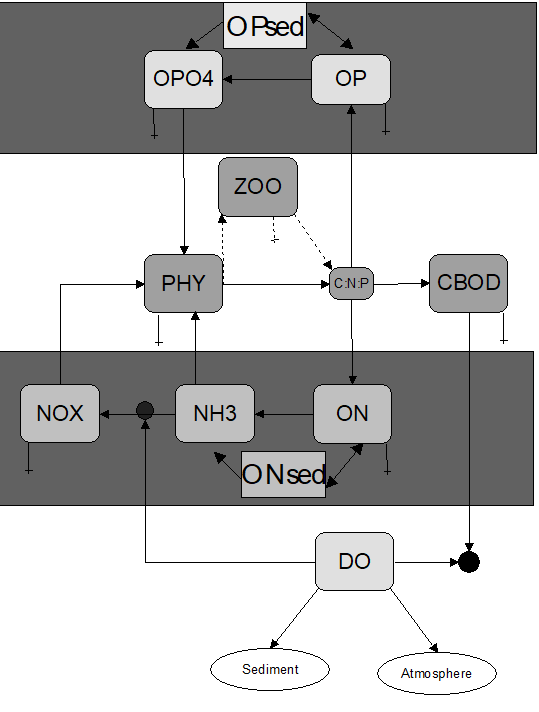
\includegraphics[scale=1]{eutro.png}
\caption{The overall structure of the EUTRO module with state variables (grey boxes), fluxes of matter (arrows). Black circles represent oxygen consumption in nitrification and in the degradation of organic matter. }
\label{eutro_scheme}
\end{figure}

The model implementation allows to vary the represented complexity, by switching the state variables on and off.
Phytoplankton (Table 1) is driven by the anabolic and the catabolic terms, plus a grazing term related to zooplankton concentration (Reaction 10, 11 and 14, \Ttwoa). The anabolic term is related to light intensity, temperature and concentration of nutrients in water, while the catabolic term depends on temperature (\Ttwoa) .
Phytoplankton growth is described by combining a maximum growth rate under optimal conditions, and a number of dimensionless factors, each ranging from 0 to 1, related to specific environmental factors (nutrient, light availability), reducing the phytoplanktonic growth when environmental conditions are suboptimal. Inorganic phosphorous and nitrogen availability on phytoplankton growth/nutrients uptake is simulated by means of Michealis-Menten-Monod kinetics (Table 2). Phytoplankton uptake nitrogen both in the forms of ammonia and nitrate, but ammonia is assimilated preferentially, as indicated in the ammonia preference relation (Reaction. 35, \Ttwoa). Temperature influence on phytoplankton growth is expressed using an exponential relation (Reaction 10, \Ttwoa), light limitation can be chosen between two alternative options (Di Toro and Smith subroutines, Reaction 41, \Ttwoa). 
Nitrogen and phosphorous are then returned to the organic compartment (ON, OP) via phytoplankton and zooplankton respiration and death. After mineralization, the organic form is again converted in the dissolved inorganic form available for phytoplankton growth. 
The DO mass balance is influenced by the reareation rate, due to the exchange with the atmosphere, and photosynthesis (sources of DO) and by respiration and mineralization of particulated and dissolved organic matter (sinks of DO). Other terms included in the DO mass balance are the ones referring to redox reactions such as nitrification and denitrification. The reaeration rate is computed taking into account the wind and current speeds, depth and temperature.
The dynamic of a generic pool of herbivorous zooplankton is simulated with the variable ZOO. Zooplankton grazing has been described by means of a type II functional relationship.
Grazed phytoplankton is assimilated according to the efficiency coefficient EFF. The not assimilated fraction is transferred to the organic matter compartments. Finally, zooplankton mortality is described by a first order kinetics. 


%------------------------------------------------------------------------
%
%    Copyright (C) 1985-2020  Georg Umgiesser
%
%    This file is part of SHYFEM.
%
%    SHYFEM is free software: you can redistribute it and/or modify
%    it under the terms of the GNU General Public License as published by
%    the Free Software Foundation, either version 3 of the License, or
%    (at your option) any later version.
%
%    SHYFEM is distributed in the hope that it will be useful,
%    but WITHOUT ANY WARRANTY; without even the implied warranty of
%    MERCHANTABILITY or FITNESS FOR A PARTICULAR PURPOSE. See the
%    GNU General Public License for more details.
%
%    You should have received a copy of the GNU General Public License
%    along with SHYFEM. Please see the file COPYING in the main directory.
%    If not, see <http://www.gnu.org/licenses/>.
%
%    Contributions to this file can be found below in the revision log.
%
%------------------------------------------------------------------------

%\documentclass{report}
%\usepackage{a4}
%\usepackage{shortvrb}
%\begin{document}



\newcommand{\Otwo}{O${}_{2}$}
\newcommand{\Degree}{${}^{o}$}
\newcommand{\power}[1]{${}^{#1}$}

\newcommand{\opn}{ {} }


\newcommand{\VSPGB}{\vspace{0.2cm}}
\newcommand{\HSP}{\hspace*{1.5cm}}
\newcommand{\HHSP}{\hspace*{0.5cm}}
\newcommand{\GBox}[2]{\parbox{#1 cm}{\VSPGB#2\VSPGB}}
\newcommand{\GDBox}[1]{\GBox{5}{#1}}
\newcommand{\GEBox}[1]{\GBox{7}{#1}}
\newcommand{\GFBox}[1]{\GBox{7}{#1}}



\begin{table}\centering
\begin{tabular}{lll}
\hline


& & \\
$\frac{\partial S}{\partial t} =Q(S)$
& &
General Reactor Equation
\\
& & \\

$Q(PHY) = GPP - DPP - GRZ$
& 1 & 
Phytoplankton PHY [mg C/L]
\\

$Q(ZOO) = GZ - DZ$
& 2 &
Zooplankton ZOO [mg C/L]
\\

$Q(NH3) = N_{alg1} + ON1 - N_{alg2} - N1$
& 3 &
Ammonia NH3 [mg N/L]
\\

$Q(NOX) = N1 - NO_{alg} - NIT1$
& 4 &
Nitrate NOX [mg N/L]
\\

$Q(ON) = ON_{alg} - ON1$
& 5 &
Organic Nitrogen ON [mg N/L]
\\

$Q(OPO4) = OP_{alg1} + OP1 - OP_{alg2}$ 
& 6 &
\GBox{5}{
Inorganic Phosphorous OPO4 \\
\HHSP [mg P/L]
}
\\

$Q(OP) = OP_{alg3} - OP1$
& 7 &
Organic Phosphorous OP [mg P/L]
\\

$Q(CBOD) = C1 - OX - NIT2$
& 8 &
\GBox{5}{
Carbonaceous Biological Oxygen \\
\HHSP Demand CBOD [mg \Otwo/L]
}
\\

\GBox{6}{
$Q(DO) = DO1 + DO2 + DO3 $\\
\HSP $\opn - DO4 - N2 - OX - SOD$
}
& 9 &
Dissolved Oxygen DO [mg \Otwo/L]
\\


\hline
\end{tabular}
\caption{Mass balances}
\label{MassBalance}
\end{table}






\begin{table}\centering
\begin{tabular}{lll}
\hline


$GPP=GP1*PHY $
& 10 &
phytoplankton growth
\\

$DPP=DP1*PHY $
& 11 &
phytoplankton death 
\\

$GRZ=KGRZ*\frac{PHY}{PHY+KPZ}*ZOO$
& 12 &
grazing rate coefficient
\\

$GP1=L_{nut} *L_{light} *K1C*K1T^{(T-T_{0} )} $
& 13 &
\GDBox{
phytoplankton growth rate with nutrient and light limitation
}
\\

$DP1=RES+K1D$ 
& 14 &
\GDBox{
phytoplankton respiration and death rate
}
\\

$GZ=EFF*GRZ$ 
& 15 &
zooplankton growth rate
\\

$DZ=KDZ*ZOO$ 
& 16 &
zooplankton death rate
\\

$Z_{ineff} = (1-EFF)*GRZ $
& 17 &
grazing inefficiency on phytoplankton
\\

$Z_{sink} = Z_{ineff}+DZ $
& 18 &
sink of zooplankton
\\

$N_{alg1}= NC*DPP*(1-FON) $
& 19 &
source of ammonia from algal 
death
\\

$N_{alg2}=PN*NC*GPP $
& 20 &
sink of ammonia for algal growth
\\

$NO_{alg}= (1. - PN)*NC*GPP $
& 21 &
sink of nitrate for algal growth
\\

$ON_{alg}= NC*(DPP*FON+Z_{sink}) $
& 22 &
\GDBox{
source of organic nitrogen from phytoplankton and zooplankton death
}
\\

\GBox{5}{
$N1=KC_{nit} *KT_{nit}^{(T-T_{0})} *NH3$
\HSP $\opn *\frac{DO}{K_{nit}+DO}$
}
& 23 &
nitrification
\\

\GBox{5}{
$NIT1=KC_{denit} KT_{denit}^{(T-T_{0})}$
\HSP $\opn *NOX*\frac{K_{denit}}{K_{denit}+DO}$
}
& 24 &
denitrification
\\

$ON1=KNC_{\min } *KNT_{\min }^{(T-T_{0})} *ON$
& 25 &
mineralization of ON
\\

$OP1=KPC_{\min } *KPT_{\min } ^{(T-T_{0})} *OP$
& 26 &
mineralization of OP
\\

$OP_{alg1}=PC*DPP*(1. - FOP) $
& 27 &
\GDBox{
source of inorganic phosphorous from algal death
}
\\

$OP_{alg2}=PC*GPP $
& 28 &
\GDBox{
sink of inorganic phosphorous for algal growth
}
\\

$OP_{alg3}=PC*(DPP*FOP+Z_{sink}) $
& 29 &
\GDBox{
source of organic phosphorous from phytoplankton and zooplankton death
}
\\

\GBox{5}{
$OX=KDC*KDT^{(T-T_{0} )} $
\HSP $\opn *CBOD*\frac{DO}{KBOD+DO} $
}
& 30 &
oxidation of CBOD
\\

\hline
\end{tabular}
\caption{Functional Expression Description}
\label{FuncDesc}
\end{table}

\begin{table}\centering
\begin{tabular}{lll}
\hline

$C1=OC*(K1D*PHY+Z_{sink}) $
& 31 &
\GDBox{
source of CBOD from phytoplankton and zooplankton death
}
\\

$NIT2=\left( \frac{5}{4} *\frac{32}{14} *NIT1\right) $
& 32 &
sink of CBOD due to denitrification
\\

$DO1=KA*(O_{sat} - DO) $
& 33 &
reareation term
\\

$DO2=PN*GP1*PHY*OC $
& 34 &
\GDBox{
dissolved oxygen produced by phytoplankton using NH3
}
\\

\GBox{5}{
$DO3=(1-PN)*GP1*PHY$
\HSP $\opn * 32*\left( \frac{1}{12} +1.5*\frac{NC}{14} \right) $
}
& 35 &
growth of phytoplankton using NOX
\\

$DO4 = OC*RES*PHY$ 
& 36 &
respiration term
\\

$N2=\left( \frac{64}{14} *N1\right) $
& 37 &
oxygen consumption due to nitrification
\\

\GBox{6}{
$PN=\frac{NH3*NOX}{(KN+NH3)*(KN+NOX)}$ 
\HSP $\opn +\frac{NH3*KN}{(NH3+NOX)*(KN+NOX)} $
}
& 38 &
ammonia preference
\\

$RES=K1RC*K1RT^{(T-T_{0})} $
& 39 &
algal respiration
\\

$SOD=\frac{SOD1}{H} *SODT^{(T-T_{0})} $
& 40 &
sediment oxygen demand
\\

$L_{nut}= min(X1,X2) \, , \,  mult(X1,X2) $
& 41 &
\GDBox{
minimum or multiplicative nutrient limitation for phytoplankton growth
}
\\

$X1=\frac{NH3+NOX}{KN+NH3+NOX} $
& 42 &
\GDBox{
nitrogen limitation for phytoplankton growth
}
\\

$X2=\frac{OPO4}{\frac{KP}{FOPO4} +OPO4} $
& 43 &
\GDBox{
phosphorous limitation for phytoplankton growth
}
\\

$L_{light} =\frac{I_{0} }{I_{s} } *e^{-(KE*H)} *e^{(1-\frac{I_{0} }{I_{s}
} *e^{(-KE*H)} )} $
& 44 &
\GDBox{
light limitation for phytoplankton growth
}
\\

$KA=F(Wind,Vel,T,T_{air},H) $
& 45 &
re-areation coefficient 
\\


\hline
\end{tabular}
\addtocounter{table}{-1}
\caption{(continued) Functional Expression Description}
\label{FuncDesc1}
\end{table}













\begin{table}\centering
\begin{tabular}{ll}
\hline


$K1D=0.12$ day\power{-1}  
&
phytoplankton death rate constant
\\

$KGRZ=1.2$ day\power{-1}  
&
grazing rate constant
\\

$KPZ=0.5$ mg C/L 
&
\GFBox{
half saturation constant for phytoplankton in grazing
}
\\

$KDZ=0.168$ day\power{-1} 
&
zooplankton death rate
\\

$K1C=2.88$ day\power{-1} 
&
phytoplankton growth rate constant
\\

$K1T=1.068$ 
&
\GFBox{
phytoplankton growth rate temperature constant
}
\\

$KN=0.05$ mg N/L 
&
\GFBox{
nitrogen half saturation constant for phytoplankton growth
}
\\

$KP=0.01$ mg P/L 
&
\GFBox{
phosphorous half saturation constant for phytoplankton growth
}
\\

$KC_{nit}=0.05$ day\power{-1} 
&
nitrification rate constant
\\

$KT_{nit}=1.08$ 
&
nitrification rate temperature constant
\\

$K_{nit}=2.0$ mg \Otwo/L 
&
half saturation constant for nitrification
\\

$KC_{denit}=0.09$ day\power{-1} 
&
denitrification rate constant
\\

$KT_{denit}=1.045$ 
&
denitrification rate temperature constant
\\

$K_{denit}=0.1$ mg \Otwo/L 
&
half saturation constant for denitrification
\\

$KNC_{min}=0.075$ day\power{-1} 
&
mineralization of dissolved ON rate constant
\\

$KNT_{min}=1.08$ 
&
\GFBox{
mineralization of dissolved ON rate temperature constant
}
\\

$KDC=0.18$ day\power{-1}
&
oxidation of CBOD rate constant
\\

$KDT= 1.047$ 
&
oxidation of CBOD rate temperature constant
\\

$NC=0.115$ mg N/mg C 
&
N/C ratio
\\

$PC=0.025$ mg P/mg 
&
C P/C ratio
\\

$OC=32/12$ mg \Otwo/mg C 
&
O/C ratio
\\

$EFF=0.5$ 
&
grazing efficiency
\\

$FON=0.5$ 
&
fraction of ON from algal death
\\

$FOP=0.5$ 
&
fraction of OP from algal death
\\

$FOPO4=0.9$ 
&
fraction of dissolved inorganic phosphorous
\\

$KPC_{min}=0.0004$ day\power{-1}  
&
mineralization of dissolved OP rate constant
\\

$KPT_{min}=1.08$ 
&
\GFBox{
mineralization of dissolved OP rate temperature constant
}
\\

$KBOD=0.5$ mg \Otwo/L
&
CBOD half saturation constant for oxidation
\\

$K1RC=0.096$ day\power{-1}  
&
algal respiration rate constant
\\

$K1RT=1.068$ 
&
algal respiration rate temperature constant
\\

$I_{s}=1200000$ lux/day
&
\GFBox{
optimal value of light intensity for phytoplankton growth
}
\\

$KE=1.0$ m\power{-1}
&
light extinction coefficient
\\

\GBox{5}{
$SOD1=2.0$ mg \Otwo/L \\
\HSP day\power{-1} m 
}
&
sediment oxygen demand rate constant
\\

$SODT=1.08$ 
&
sediment oxygen demand temperature constant
\\

$T_{0}=20$ \Degree C 
&
optimal temperature value
\\


\hline
\end{tabular}
\caption{Parameters}
\label{Paras}
\end{table}





\begin{table}\centering
\begin{tabular}{lll}
\hline


$T$ 
& [\Degree C] &
water temperature
\\

$T_{air}$ 
& [\Degree C] &
air temperature
\\

$O_{sat}$  
& [mg/L] &
DO concentration value at saturation
\\

$I_{0}$ 
& [lux/day] &
incident light intensity at the surface
\\

$H$ 
& [m] &
depth
\\

$Vol$ 
& [m\power{3}] &
volume
\\

$Vel$ 
& [m/sec] &
current speed
\\

$Wind$ 
& [m/sec] &
wind speed
\\


\hline
\end{tabular}
\caption{Variables}
\label{Vars}
\end{table}




%\end{document}



\subsubsection{sediment module}
An additional process that can be switched on and off is the evolution of both nitrogen and phosphorus detritus in sediment. The variables  ONsed and OPsed (not subjected to advection-diffusion processes) are used in this case. These two variables interact with the Nitrogen and Phosphorous cycles through the resuspension and sinking of organic N and P, as described by the equations in Table 1. When the wsedim  subroutine is switched on, OP, ON, NH3 and OPO4 are updated at each time step in agreement with those equations. The resuspension is a linear function of the water velocity calculated by the hydrodynamic model at each box, as written in Tab. \ref{MassBalance}. The amount of the sinking nutrients depends on specific parameters, as given in Tab. \Ttwoa, and on the depth of the underlying column.
This routine can be switched on and off as needed by the user, setting the |bsedim|, parameter true or false in the bio3d routine. 

\subsubsection{Parameters for the str file}
Below the parameters to set in the input file |str|


|Ibio=1|		simulate eutro

To set boundary conditions add a section |$bound| and set:

|bio2dn=| File name that contains boundary conditions for concentration of the water quality state variables. The format is the same as for the file boundn. The unit of the values given in the second and following column (9 data columns for EUTRO) must the ones of the variable.

Initialization of variables are done using external files, otherwise are set by default in the code, with uniform value in the domain.  Spatially variable initial conditions should be provided in section |$name|.
\begin{itemize}
\item Name1.bio: File with concentration values of water quality for the initialization.
\item Name1.salt: Files with salinity concentration values [psu] for the initialization.
\item Name1.temp: File with and Temperature values [deg C] for the initialization.
\end{itemize}

%For further details about EUTRO-WASP integration into SHYFEM see \cite{Umgie2003}.


%\subsubsection{ERSEM-BFM}

%The ecosystem model is built on the base of the Biogeochemical Flux Model (ERSEM-BFM), a biomass-based differential equation model. The model is built with respect to mass conservation following a top-down approach, where the food web consists of functional groups defined as Chemical Functional Families and Living Functional Groups. Each group is expressed in terms of basic elements components, such as C, N, P and SI, or by molecules as Chlorophyll, which constitutes a set of state variables. The model simulates the evolution of up to 44 state variables in the water column describing both the main metabolic processes within each functional groups and the predation processes between functional groups. In particular, carbon assimilation, nutrient uptake, analysis of primary producers, grazing by and of secondary producers, respiration, mortality excretion and exudation of all organisms are modelled.

%Only the pelagic foodweb has been considered which is constituted by primary producers, zooplankton, bacteria, nutrients and dissolved chemical species for oxygen and the carbonate system. Primary producers are divided in four principal groups: one silicate dependent group named diatoms and three silicate independent groups named picophytoplankton, flagellates and dinoflagellates. Bacterioplankton represent free-living, non-colonial bacteria that can switch from aerobic to anaerobic metabolism according to the pelagic oxygen conditions. There are four zooplankton groups in the model corresponding to microzooplankton, heterotrophic nanoflagellates, carnivorous mesozooplancton and omnivorous mesozooplancton. The other explicitly simulated environmental variables are nutrients (nitrite, nitrate, ammonium, orthophosphate and silicate. dissolved bioavailable iron), dissolved oxygen, carbon dioxide, dissolved and particulate (non-living) organic matter.

%More information on the ERSEM-BFM ecological module can be found at https://www.nioz.nl/en/about/cos/ecosystem-modelling/ersem-bfm-model